\documentclass{article}
\usepackage{tabulary}
\usepackage{amsmath,esint}
\usepackage{amssymb}
\usepackage{amsthm}
\usepackage{bm}
\usepackage{graphicx}
\usepackage[utf8]{inputenc}
\usepackage{cleveref}
\usepackage{biblatex}
\usepackage{subcaption}

\def\rcurs{{\mbox{$\resizebox{.16in}{.08in}{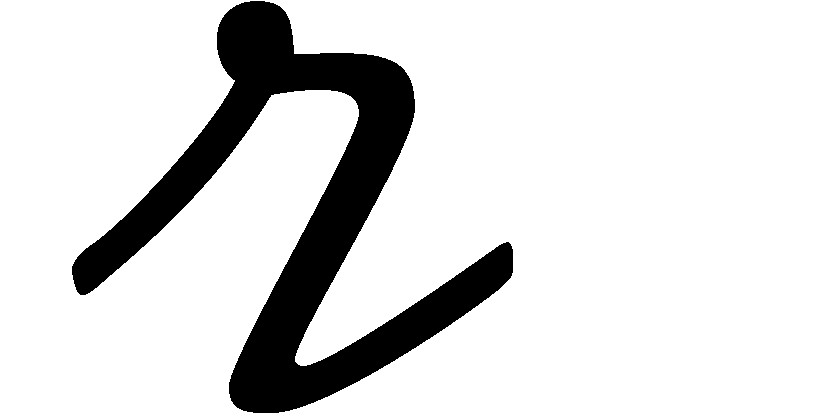
\includegraphics{ScriptR}}$}}}
\def\brcurs{{\mbox{$\resizebox{.16in}{.08in}{
\includegraphics{BoldR}}$}}}
\def\hrcurs{{\mbox{$\hat \brcurs$}}}

\author{Alex Seewald}
\title{Mathematical Physics Independent Project Paper}
\addbibresource{sources.bib}
\begin{document}

\newcommand{\unit}[1]{ \hat{\mathbf{e}_{#1}} }
\newcommand{\skewunit}[1]{ \hat{\mathbf{g}_{#1}} }
\newcommand{\partialfrac}[2]{\frac{\partial{#1}}{\partial{#2}}}
\newcommand{\norm}[1]{\lvert #1 \rvert}

\nocite{*}


\maketitle

\tableofcontents

\section*{Introduction}

Most high school students have a go-to coordinate system and physists have at least three. Although using familiar coordinate systems is cognitively automatic, it is deep when one pays close attention to the process. A coordinate system creates a correspondence between what is “there” and a representation of that location. The symbolic expression of this correspondence is a dot product between a representation (components) and basis elements. Not only is that correspondence internally consistent, but any coordinate system’s representation can be transformed into a representation in another coordinate system of equal dimensionality. That is, while it is common to think about rectangular coordinates as the fundamental coordinate system and other coordinate systems as being defined in terms of rectangular coordinates for the sake of making certain problems more convenient, there is nothing more fundamental about rectangular coordinates.

%these hrefs should be hyper-references to places in my paper.
Much of the knowledge people pick up in calculus is local to the rectangular coordinate system. There are, however, more general and verbose specifications of ideas like 'curl'. To reduce this verbosity, many texts use a taxonomy of 'orthogonal vs non-orthogonal', 'unit-basis vs non-unit-basis', and 'position-independent vs position-dependent' \footnote{I use $q_i$ to signify an orthogonal, curvilinear component and $g_i$ to signify a non-orthogonal component in the tradition of Kusse and Westwig}. There is not, as far as I know, some flow-chart-like procedure for choosing the most convenient coordinate system for a problem. The way to get that convenience seems to be learning about coordinate systems in general, and then having insights. One source of convenience is that one can exploit symmetries (see notebook). Another is that there are physical situations that people approach as a standalone problem, e.g. the Lorentz transform, that can be thought of as instances of a coordinate system problem (see notebook). While this is more of a curiosity than a convenience, the coordinate system problem also includes the problem of changing units, e.g. adjusting from inches to centimeters. Fortunately, this is reflected in the word 'unit' as meaning 'the amount corresponding to the number 1', just as a unit vector is an amount corresponding to '1'.

\section*{Orthogonal Coordinate Systems}

It is sufficient in specifying a coordinate system to define each coordinate value as a function of coordinate values in another system. Orthogonal systems have the property of orthogonal basis vectors at every point, expressed $\unit{i} \cdot \unit{j} = \delta_{i,j}$, with the Kronecker delta symbol. Four such systems are the toroidal coordinate system, a change from inches to centimeters and change from footpounds to joules, a linear change of basis, and an insubstantial substitution:

\begin{align*}
x &= a sinh(\eta) * cos(\phi) / (cosh(\eta) - cos(\zeta)) & x &= 2.54 x'  & x &= 0.6 x' + 0.1 y' & x &= y'\\
y &= a sinh(\eta) * sin(\phi) / (cosh(\eta) - cos(\zeta)) & y &= 1.36 y'  & y &= 0.2 x' + 0.7 y' & y &= z' \\
z &= a sin(\zeta) / (cosh(\eta) - cos(\zeta))             & z &= z'       &                      & z &= x' \\
\end{align*}

It is sufficient to specify these coordinate functions because a coordinate consists of components and basis vectors, and the component functions can be used to generate basis vectors. This process is outlined in \cref{tab:orth}. A potentially surprising consequence of this definition is that unit vector definitions are \textit{associated with} a point, rather than having a single identity that is applied at every point. However, this result passes the sanity check of $\unit{r}$ pointing from the origin to the point in spherical coordinates, wherever that point is. Scaling factors are the parameters of expressing vector calculus ideas in arbitrary curvilinear coordinates; for an example of a derivation of such a general result \cref{sec:curl}, for a full list of such results see \cref{tab:orth}. Because scaling factors are a relative concept, there must be a starting place. The idea is that two position-independent unit vectors have '1' as the relative value, e.g. (why is scaling factor of radius 1?)

Kusse and Westwig present the unit vectors as emerging from equations relating one coordinate system to another. This inductive definition would not be able to generate coordinate systems if there were not an base-case coordinate system whose unit vectors are already known. The soundness of this approach, then, depends on the existence of at least one coordinate system which can be thought of without this framework. Rectangular, cylindrical, and spherical coordinate systems are all widely-used and intuitive to physicists, so there is not a base-case problem.

\begin{table}
\begin{tabulary}{\textwidth}{|L|L|}
\hline
Name & Definition \\
\hline
Representation  & $ q_i = q_i(x,y,z) $ \\
as usually done & $ x = X(q_1,q_2,q_3), y = Y(q_1,q_2,q_3), z=Z(q_1,q_2,q_3) $\\
\hline
Basis as usually done & $ \hat{q_i} = \frac{\partial{\textbf{r}} / \partial{q_i}}{h_i} $\\
& Here, r is a vector of rectangular coordinates \\
\hline
Representation  & $q_i = q_i(q'_1,q'_2,q'_3) $ \\
in general      & $q'_i = q_i'(q_1,q_2,q_3) $ \\
\hline
Basis in general & $ \hat{q_i} = \frac{\partial{\textbf{r}} / \partial{q_i}}{h_i / h_j} $ \\
& Here, r is a vector of curvilinear coordinates \\
\hline
Scaling Factor & $ h_i = \norm{\partialfrac{\textbf{r}}{q_i}} $ \\
\hline
Dot Product & $  \textbf{U} \cdot \textbf{V} = U_i B_j \delta_{i,j} = U_i V_i $\\
\hline
Gradient & $\nabla \Phi = \frac{1}{h_i} \partialfrac{\Phi}{q_i} \hat{q_i} $ \\
& where $\Phi$ is some scalar function. \\
\hline
Path Integral & $ \int_{C} d\textbf{r} \cdot \textbf{V} = \int_{C} dq_1 h_1 V_1 + dq_2 h_2 V_2 + dq_3 h_3 V_3  $ \\ 
& where the vector is of same coordinate system as integral body. \\
\hline
Surface Integral & $ \iint_{S} d {\bm \sigma} \cdot \textbf{V} = \iint_{S} \pm dq_1 dq_2 h_1 h_2 V_3 +
                                                                           \pm dq_1 dq_3 h_1 h_3 V_2 +
                                                                           \pm dq_2 dq_3 h_2 h_3 V_1 $ \\
& where sign is sign of d $ {\bm \sigma} \cdot \unit{q_i}$ \\
\hline
Volume Integral & $\iiint_{\tau} dq_1 dq_2 dq_3 h_1 h_2 h_3 \rho(q_1,q_2,q_3) $ \\
& where $\rho$ is some scalar function with a density-like meaning. \\
\hline
Divergence & $ \nabla \cdot \textbf{U} = \frac{1}{h_1 h_2 h_3} (\frac{\partial{h_2 h_3 U_1}}{\partial{q_1}} +
                                                                \frac{\partial{h_3 h_1 U_2}}{\partial{q_2}} +
                                                                \frac{\partial{h_3 h_2 U_3}}{\partial{q_3}}) $ \\
\hline
\end{tabulary}
Curl : $\nabla \times \textbf{U} = \frac{1}{h_1 h_2 h_3}  \begin{vmatrix}
                                                     h_1 \hat{q_1} & h_2 \hat{q_2} & h_3 \hat{q_3} \\
                                                     \partialfrac{ }{q_1} & \partialfrac{ }{q_2} & \partialfrac{ }{q_3} \\
                                                     h_1 U_1 & h_2 U_2 & h_3 U_3 \\
                                                     \end{vmatrix} $ \\
\caption{These ideas are laid out in 3 dimensions for sake of being visualizable.}
\label{tab:orth}
\end{table}

\section*{Qualitative Discussion of Orthogonal Curvilinear Coordinate Systems}

Until I did this project, I had never heard that cylindrical and spherical coordinates constitute an orthogonal coordinate systems and did not have a visual picture of how they are orthogonal. With cylindrical coordinates, $\unit{z}$ always points upwards, so $\unit{\phi}$ and $\unit{\rho}$ are constrained to a constant z plane. $\unit{\rho}$ points in the direction of the projection of the component vector $\textbf{r}$ onto the plane. $\unit{\phi}$ is position-dependent, and thought of as being always perpendicular the other two vectors. With spherical coordinates, $\unit{r}$ points in the same direction as the component vector $\textbf{r}$. $\unit{\theta}$ and $\unit{\phi}$ are, then, constrainted to within the plane normal to that vector. $\unit{\theta}$ is visualized such that if $\theta$ has value L degrees, it points L degrees above a plane of constant 'z'. This dependence of the direction on the value is what is meant by position dependence.

Elliptical cylindrical coordinates have the surfaces of constant $u$ being ellipses with foci at $(a,0), (-a,0)$ in rectangular coordinates, where increasing values of $u$ corresponding to ellipses of greater area. $\unit{u}$ is thought as perpendicular to that ellipse, and in a constant-z plane. The surfaces of constant $v$ are hyperbolas centered around the origin, where the value of $v$ is the angle from the x axis that the hyperbola approaches as its behavoir approaches a line. $\unit{v}$ is thought of as pointing along the contour of the elliptical surface of the point. Collectively, $u$ and $v$ specify a point in a plane, so another coordinate $z$ specifies which plane in $\mathbb{R}^3$.

\begin{figure}
    \centering
    \begin{subfigure}[b]{0.3\textwidth}
        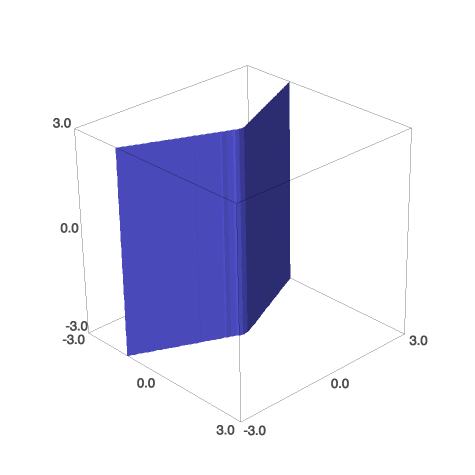
\includegraphics[width=\textwidth]{images/spherical_phi.png}
        \caption{constant phi in spherical}
    \end{subfigure}
    \begin{subfigure}[b]{0.3\textwidth}
        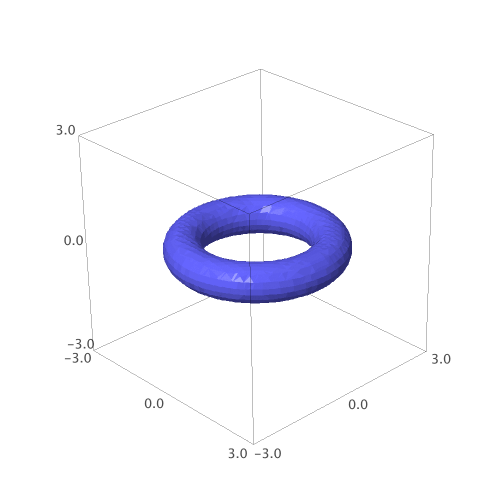
\includegraphics[width=\textwidth]{images/toroidal_tau.png}
        \caption{constant tau in toroidal}
    \end{subfigure}
    \begin{subfigure}[b]{0.3\textwidth}
        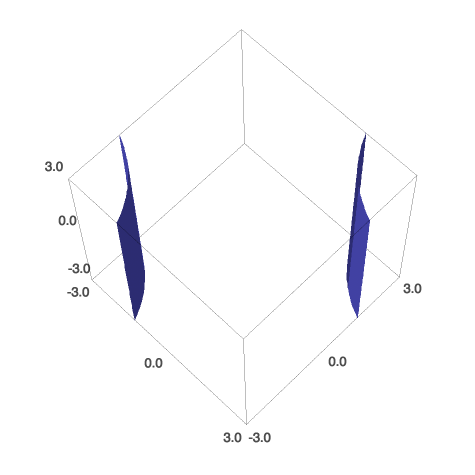
\includegraphics[width=\textwidth]{images/hyperbolic_v.png}
        \caption{constant v in hyperbolic-cylindrical}
    \end{subfigure}
\caption{Isosurfaces}
\end{figure}

\begin{figure}
    \centering
    \begin{subfigure}[b]{0.3\textwidth}
        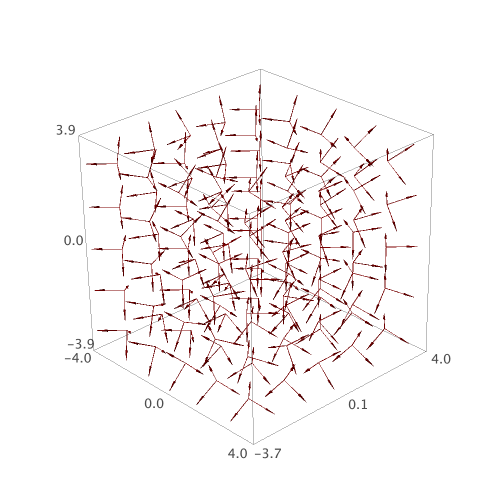
\includegraphics[width=\textwidth]{images/spherical_bases.png}
        \caption{spherical}
    \end{subfigure}
    \begin{subfigure}[b]{0.3\textwidth}
        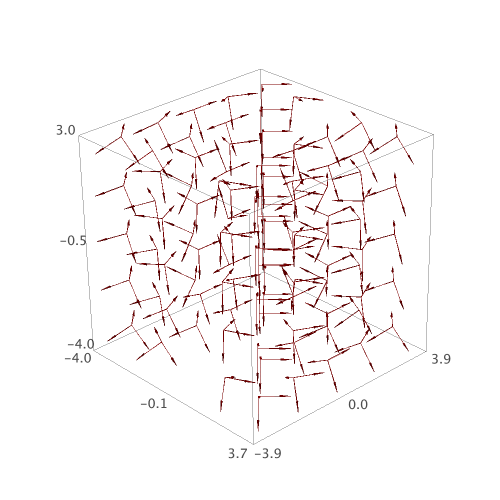
\includegraphics[width=\textwidth]{images/toroid_bases.png}
        \caption{toroidal}
    \end{subfigure}
    \begin{subfigure}[b]{0.3\textwidth}
        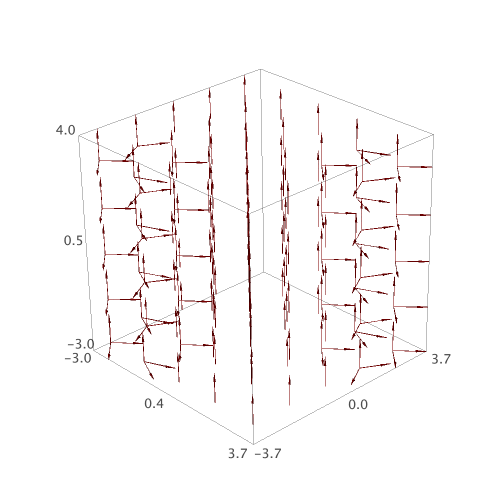
\includegraphics[width=\textwidth]{images/hyperbolic_bases.png}
        \caption{hyperbolic-cylindrical}
    \end{subfigure}
\caption{Unit Basis Vectors}
\end{figure}


\section*{Applications of Orthogonal Coordinate Systems}
\label{sec:convenient}

Imagine a uniform distribution of charge in an elliptical cylinder of major axis 2, minor axis 1, and height 3. Given a surface, Gauss' Law relates the resulting electric field to the charge enclosed within the surface. The integral body is easiest to evaluate when $d \textbf{A}$ and $\textbf{E}$ are always parallel, so one chooses the surface where $z$ goes from 0 to 4 and $v$ goes from 0 to a large number, and $\mu$ is some value such that all charge is contained (such as 3). In order to accomodate major axis 2 and minor axis 1, using the property of ellipses relating foci distance to axes lengths: $a = \sqrt{2^2 - 1^2} = \sqrt{3}$. With this coordinate system and surface:

\begin{align*}
\frac{Q_{enc}}{\epsilon_0} &= \oiint \textbf{E} \cdot d \textbf{A} \\
\frac{\rho * \pi * 1 * 2 * 3}{\epsilon_0} &= \int_{v=0}^{2 \pi} \int_{z=0}^{4} E dq_v dq_z h_v h_z \\
\frac{\rho * 6 \pi}{\epsilon_0} &= \int_{v=0}^{2 \pi} \int_{z=0}^{4} E dq_v dq_z \sqrt{3} \sqrt{sinh^2(3) + sin^2(v)} 1 \\
E &= \unit{\mu} \frac{\rho * 6 \pi}{\epsilon_0 4 \sqrt{3} \int_{v=0}^{2 \pi} dq_v \sqrt{sinh^2(3) + sin^2(v)}} 
\end{align*}

The integral for this expression of the value of $E$ along the surface complicated, and best evaluated with a numerical method. While the introduction of the $v$ scaling factor does not feel convenient, using elliptical cylindrical coordinates allowed for the symmetry that permits $E$ to be assumed a constant along with surface and therefore extractable from the integral.

As far as I know, there is no easy way to express vector addition in curvilinear coordinates. The whole head-to-tail procedure relies on position-independence, which is not in general guaranteed. Some physical problems that have a symmetry one would like to have reflected in the coordinate system, but also have the notion of vector addition. The way to handle this is to do different subproblems in different coordinate systems, and convert results into a common system. The Ampere's Law in Griffith's \textit{Introduction to Electrodynamics} shows this process \cite{griffiths}:

\section*{Coordinate System Transformations}
\label{sec:trans}

The robustness of the transformation matrix is not necessarily obvious, but it is order-independent and, when the coordinate system is orthonormal, invertible with the property $a_{i,j}^{-1} = a_{j,i}$. The order-independence of coordinate components can be thought of like so: interchange the $j$ and $j + 1$ columns of $\textbf{A}$. Because $ V'_i = \textbf{A}_{i,j} V_j $ expresses a sum over all j rows, and addition is commutative, the bindings $q_1 = \rho, q_2 = \phi, q_3 = z$ work just like the bindings $q_1 = \rho, q_2 = z, q_3 = \phi$. The invertibility property is explained like so in \cite{kusse}:

\begin{proof}
\begin{align*}
\unit{j} &= A_{i,j} \unit{i}'                                  \tag*{\small {the definition}} \\
\unit{j} \cdot \unit{k} &= A_{i,j} (\unit{i}' \cdot \unit{k})  \tag*{\small {same operation to both sides}} \\
\delta_{j,k} &= A_{i,j} A_{i,k}                                \tag*{\small {substitution definition of Kronecker delta}} \\
A A^T &= [1]                                                   \tag*{\small {Matrix of Kronecker delta values \textit{is} identity matrix}} \\
\end{align*}
\label{proof:invert}
\end{proof}

Because the definition of the Jacobian is $ [\frac{\partial{\textbf{F}}}{\partial{q_1}}  \frac{\partial{\textbf{F}}}{\partial{q_2}} ... \frac{\partial{\textbf{F}}}{\partial{q_n}} ]$, this transformation matrix can be thought of as a Jacobian if $\textbf{F}$ is thought to be a vector of curvilinear components as a function of other curvilinear components.

\begin{table}
\begin{tabulary}{\textwidth}{|L|L|}
Name & Definition \\
Transform Matrix & $\textbf{A}_{i,j} = \frac{h'_i \partial{q_i'(q_1,q_2,q_3)}}{h'_j \partial{q_j}} $\\
\hline
Transform & $V'_i = \textbf{A}_{i,j} V_j, $\\
\hline
Reverse Transform & $V_j = \textbf{A}_{j,i} V'_i, $\\
\hline
\end{tabulary}
\caption{This table is a summary of results described in Mathematical Physics by Kusse and Westwig, and uses their implicit summation notation. That is, the transformation matrix row here expresses a sum of partial derivatives for all $x_j$ in the range.}

\label{tab:transform}
\end{table}

\section*{Non-Orthogonal Coordinate Systems}

Like how the study of non-rectangular, orthogonal coordinate systems introduces the concept of scaling factors to allow for a generalization of vector calculus operations, the study of non-orthogonal coordinate systems introduces the concept of covariance and contravariance of vectors. The covariant components of a vector are a rewriting of the familiar, now called contravariant, components that follow dot product rules with non-orthogonal bases. The rewriting rule is $A_i = A^j (\hat{g_i} \cdot \hat{g_j})$, where superscripts indicate a contravariant component, and subscripts a covariant component. If $B_1 = B^1 + B^2 (\hat{g}_1 \cdot \hat{g}_2), B_2 = B^1(\hat{g}_1 \cdot \hat{g}_2) + B^2$, then $\textbf{A} \cdot \textbf{B} = A^1 B_1 + A^2 B_2$. 

The explanation of the coordinate transformation matrix inversion in \cref{proof:invert} relied on the Kronecker delta describing dot products of the bases. However, the Kronecker delta does not fit non-orthogonal coordinate systems because $\hat{g}_i \cdot \hat{g}_j \neq 0$ is what is meant by non-orthogonality. The way to produce the inverse is, then, to just build it up from the relevant partial derivatives as one does to produce the original:

\begin{table}
\begin{tabulary}{\textwidth}{|L|L|}
Name & Description \\
Contravariant Transform & $t_{i,j} = \partialfrac{x^i'}{x^j} $ \\
& $t_{i,j}^{-1} = \partialfrac{x^i}{x^j'} $ \\
& $V^i' = t_{i,j} V^j, \hat{g}_j' = t_{i,j} \hat{g}_i $ \\
\hline
\hline
 & $ {\bm \beta} = \frac{1}{c} \textbf{v}$ \\
\hline
 & $ \gamma = \frac{1}{\sqrt{1 - {\bm \beta} \cdot {\bm \beta}}} $\\
\hline
General Lorentz Transform & $ \textbf{T}_{i,j} = (\gamma - 1) \frac{ \beta_i \beta_j}{\norm{\beta}^2 } + \delta_{i,j}$ \\ 
\hline
\end{tabulary}

Skewed Bases: $\begin{pmatrix} 
               \skewunit{1}' & \skewunit{2}' 
               \end{pmatrix} 
               = 
              \begin{pmatrix} 
              \skewunit{1} & \skewunit{2} 
              \end{pmatrix} \textbf{T}^{-1}$

Special cases of Lorentz Transform with x-only velocity between frames:

$\textbf{T} = \begin{pmatrix}
              \gamma & - \gamma \beta \\
              - \gamma \beta & \gamma \\
              \end{pmatrix} , 
\textbf{T} = \begin{pmatrix}
              \gamma & 0 & 0 & - \gamma \beta \\
              0 & 1 & 0 & 0 \\
              0 & 0 & 1 & 0 \\
              - \gamma \beta & 0 & 0 & \gamma \\
              \end{pmatrix} $
\caption{ }
\label{tab:non_orth}
\end{table}

In the context of special relativity, reference frames have their own rectangular coordinate systems, one of whose components represents time. Distinct reference frames can be said to view each other's coordinate systems as non-orthogonal (\cref{fig:axes}). The physical interpretation of the non-aligned axes is relativity of simultanaity: events happening along a $t=k_1$ line do not occur along a $t'=k_2$ line. Similarly, because the position axes are not aligned, there is a relativity of position. (length contraction and time dilation discussion here).

Another way the discussion of coordinate systems systematizes thought about special relativity is through the metric tensor. A metric tensor is the parameter $g_{i,j}$ in the general definition of distance: $ (ds)^2 = g_{1,1} (dx_1)^2 + g_{1,2} dx_1 dx_2 + g_{2,2} (dx_2)^2 + ...$ \cite{mathworld}. When the Kronecker delta is used as the metric tensor, this distance definition is the familiar pythagorean theorem. However, the length of a vector in space-time is determined with the Minkowski metric:
$\begin{pmatrix}
-1 & 0 & 0 & 0 \\
0 & 1 & 0 & 0 \\
0 & 0 & 1 & 0 \\
0 & 0 & 0 & 1 \\
\end{pmatrix}$

This definition is used because it produces the four-vector: the quantity that is invariant under lorentz transformation. \cref{proof:fourVector} is a proof of the invariance for $(x,t)$ systems.

\begin{proof}
\begin{align*}
(x')^2 - (c t')^2 &= x^2 - (c t)^2 \\
&= (\gamma x - \gamma \beta c t)^2 - (- \gamma \beta x + \gamma c t)^2  \\
&= \gamma^2 x^2 (1 - \beta^2) + \gamma^2 c^2 t^2 (\beta^2 - 1) \\
&= \gamma^2 (1 - \beta^2) (x^2 - c^2 t^2) \\
&= \frac{1 - \beta^2}{1 - \beta^2} x^2 - (c t)^2 \\
\end{align*}
\label{proof:fourVector}
\end{proof}

\begin{figure}
% todo - get two plots of axes from reference frame A and reference frame B's axes from A's perspective, side by side with s/A/B/flip
%\includegraphics{ }
%\includegraphics{ }
\caption{}
\label{fig:axes}
\end{figure}

\section*{Derivation of Curvilinear Curl}
\label{sec:curl}

The derivation starts with Stoke's theorem, $ \iint_S d {\bm \sigma} \cdot \nabla \times \textbf{A} = \oint_C d\textbf{r} \cdot \textbf{A}$, and considers an infinitesimal area. The closed path around the portion of the surface where $ d {\bm \sigma} $ is parallel to $q_1$, and therefore orthogonal to $q_2$ and $q_3$, is expressed as:

\begin{multline*}
%\lim_{S \rightarrow \textbf{0}} \iint_S \sum_{i = 1}^{3} \hat{q_i} \cdot (\nabla \times \textbf{A}) h_{i+1 mod 3} h_{i + 2 mod 3} dq_{i+1 mod 3} dq_{i+2 mod 3}. \\ \\
\oint_C d\textbf{r} \cdot \textbf{A} &= \int_{q_{2_0}}^{q_{2_0} + dq_2} (dq_2 (A_2 h_2) |_{q_{2_0}, q_{3_0}} + \partialfrac{A_2 h_2}{q_2} |_{q_{2_0},q_{3_0}} (q_2 - q_{2_0})) + \\
\int_{q_{2_0} + dq_2}^{q_{2_0}} (dq_2 (A_2 h_2) |_{q_{2_0}, q_{3_0}} + \partialfrac{A_2 h_2}{q_2} |_{q_{2_0},q_{3_0}} (q_2 - q_{2_0}) + \partialfrac{A_2 h_2}{q_3} |_{q_{2_0},q_{3_0}} dq_3) + \\
\int_{q_{3_0}}^{q_{3_0} + dq_3} (dq_3 (A_3 h_3) |_{q_{2_0}, q_{3_0}} + \partialfrac{A_3 h_3}{q_3} |_{q_{2_0},q_{3_0}} (q_3 - q_{3_0})) + \\
 \int_{q_{3_0} + dq_3}^{q_{3_0}} (dq_3 (A_3 h_3) |_{q_{2_0}, q_{3_0}} + \partialfrac{A_3 h_3}{q_3} |_{q_{2_0},q_{3_0}} (q_3 - q_{3_0}) + \partialfrac{A_3 h_3}{q_2} |_{q_{2_0},q_{3_0}} dq_2) \\
 &= (A_2 h_2) |_{q_{2_0}, q_{3_0}} dq_2 + \partialfrac{(A_2 h_2)}{q_2} |_{q_{2_0}, q_{3_0}} \frac{(dq_2)^2}{2} - \\
 ((A_2 h_2) |_{q_{2_0}, q_{3_0}} dq_2 + \partialfrac{(A_2 h_2)}{q_2} |_{q_{2_0}, q_{3_0}} \frac{(dq_2)^2}{2} + \partialfrac{A_2 h_2}{q_3} |_{q_{2_0},q_{3_0}} dq_2 dq_3) + \\
 (A_3 h_3) |_{q_{2_0}, q_{3_0}} dq_3 + \partialfrac{(A_3 h_3)}{q_3} |_{q_{2_0}, q_{3_0}} \frac{(dq_3)^2}{2} - \\
 ((A_3 h_3) |_{q_{2_0}, q_{3_0}} dq_3 + \partialfrac{(A_3 h_3)}{q_3} |_{q_{2_0}, q_{3_0}} \frac{(dq_3)^2}{2} + \partialfrac{A_3 h_3}{q_2} |_{q_{2_0},q_{3_0}} dq_2 dq_3) \\
&=  dq_2 dq_3 (\partialfrac{h_3 A_3}{q_2} - \partialfrac{h_2 A_2}{q_3}) \\ \\
\end{multline*}

Substituting into Stoke's theorem, we get $\hat{q_1} \cdot \nabla \times \textbf{A} = \frac{1}{h_2}{h_3} (\partialfrac{h_3 A_3}{q_2} - \partialfrac{h_2 A_2}{q_3}) $

This integral evaluation uses the fact that $A_2 h_2$, $A_3 h_3$ and their partial derivatives are known at the point $(q_{2_0}, q_{3_0})$, and that the differential path length allows the value of $A_2 h_2$ at any point in the path to be approximated with that value plus the necessary rates of change. It also uses the differential path length to have the four branches of the path separated by points that make a square, the assumption which is neccesary to allow the last step of simplification. This process gives the $q_1$ component of the curl. Repeating the process with the portion of the surface whose normal is parallel to $q_2$ and again with $q_3$ produces the $q_2$ and $q_3$ components of the curl.

\section*{Miscellaneous}

Orthonormal coordinate systems can be constructed which have a 

$q1'(q1,q2,q3), q2'(q1,q2,q3), q3'(q1,q2,q3) $ 

form, but no straightforward way to express the components in terms of primed components. For example, the elliptical cylindrical coordinate system's relationship of $x$ and $y$ to $u$ and $v$ cannot be easily solved for $u$ or $v$:

\begin{align*}
\frac{x^2}{a^2 cosh^2 u} + \frac{y^2}{a^2 sinh^2 u} &= 1 \\
\frac{x^2}{a^2 cos^2 v} - \frac{y^2}{a^2 sin^2 v} &= 1 \\
\end{align*}

$x = sin(q_1 + q_2), y = cos(q_1 + q_2), z = q_3$ is an orthogonal coordinate system because $cos(u)$ and $sin(u)$ are orthogonal and, $q_1$ and $q_2$ are in the $\mathbb{R}^2$ subspace that touches only x and y (which is uniquely the x-y plane), and $q_3$ is an alias for $z$, so it is naturally orthogonal to that x-y plane. However, $cos$ and $sin$ have a range of $[-1,1]$, so the space spanned by $(q_1,q_2,q_3)$ is not the same as $(x,y,z)$. In addition to changing the expressable subspace, changes of coordinate system can also change uniqueness. While $\textbf{r} = (0, k_1, k_2)$ is a family of vectors that mean the zero vector in spherical coordinates, $(0,0,0)$ is the only zero vector in rectangular coordinates.

What is there to say about degrees of freedom?

\printbibliography
\end{document}
